\documentclass[12pt,letterpaper]{hmcpset}
\usepackage[margin=1in]{geometry}
\usepackage{graphicx}
\usepackage{hyperref}

% info for header block in upper right hand corner
\name{Name: \underline{\hspace{4cm}}}
\class{Math 45: Section \underline{\hspace{1cm}}}
\assignment{Assignment 3}
\duedate{3/29/18}

\begin{document}

\begin{problem}
1. (5 points) A certain drug is being administered intravenously to a hospital patient who has
had no prior drug treatments. Fluid containing $5 mg/cm^3$ of the drug enters the patient’s
bloodstream at a rate of $100 cm^3/hr$. The drug is absorbed by tissues or otherwise leaves
the bloodstream at a rate proportional to the amount present, with a rate constant of $0.4
(hr)^{-1}$.

\begin{enumerate}
    \item[(a)] Assuming that the drug is always uniformly distributed throughout the bloodstream,
write a differential equation for the amount of the drug that is present in the bloodstream
at any time and state the initial condition.
    \item[(b)] Use the integrating factor method to solve this IVP.
    \item[(c)] How much of the drug is present in the bloodstream after a long time?
\end{enumerate}

\end{problem}
\newpage

\begin{problem}
2. (10 points total: 5 points for part (a) and 5 points for parts (bcd)) Consider the DE $y' = cos(t)-y$.
\begin{enumerate}
    \item[(a)] Find the general solution to this ODE (by hand).
    \item[(b)] Generate the direction field and some solution curves for this DE with a range of
different initial conditions. Google "slope field" or "direction field" to find an app that
draws slope fields. Attach a printout with your homework.
    \item[(c)] Based on your numerical exploration in part (b), conjecture what happens to $y(t)$ as $t$
tends to infinity. Can you explain this behavior from the general solution you found in
part (a)?
    \item[(d)] If you were given the sketch of the direction field from part (a), but were not given the
equation, how would you know that the DE was non-autonomous?
\end{enumerate}
\end{problem}
\newpage

\begin{problem}
3. (10 points total: 5 points for parts (abc) and 5 points for (d)) You have been hired by a
fishery to do some preliminary work on modeling a fish population under various harvesting
strategies. They have asked you to start with this mathematical model that accounts for
logistic growth, death, and harvesting:\\

\begin{center}
    $\frac{dP}{dt}= rP(1 - P/K)-\alpha P-H(t, P)$.
\end{center}

Here, $P(t)$ represents the fishery biomass (total mass of fish). The constant $r$ relates to
the growth rate of your population, and $K$ is the carrying capacity of your fishery- the
maximum biomass that the fishery can sustain. The term -αP accounts for the natural
death of the fish. Assume $r$, $K$, $\alpha$, and $P(t)$ are all positive\\

The function $H(t, P)$ describes the harvesting of the fish. The fishery wants to understand
what would happen to the population of fish under different harvesting scenarios

\begin{enumerate}
    \item[(a)]Pick your favorite aquatic organism to model, then come up with reasonable values for
all of your parameters. What units will they have? You can try to look up values on
the Internet, or just make some reasonable estimates.
    \item[(b)] What initial condition(s) will you use? Explore how your solutions might differ with
different choices of initial condition.
    \item[(c)] First, consider harvesting strategies that are time invariant. In other words, consider
only cases where H is not a function of time. Here are two natural choices for
$H = H(P)$:

\begin{itemize}
  \item the fishery could harvest at a constant rate (say $H = 10$ kg/day)
  \item the fishery could harvest at a rate that is proportional to the fishery biomass
(e.g. $1\%$ of the biomass is harvested every month).
\end{itemize}
In each of these two cases, calculate the long-term population of the fish, and the longterm
harvesting rate. Perform these calculations by hand.

    \item[(d)] In the case where $H$ is proportional to $P$, compare the following:
    
\begin{itemize}
  \item Solve for $P(t)$ analytically (by hand)
  \item Numerically approximate $P(t)$ using Euler’s Method, twice with different time
steps. You may use a spreadsheet, Python, MATLAB, or other computer methods
to perform Euler’s method. (Use MATLAB’s ode45 numerical DE solver to
approximate P(t). We are providing code for you to run in MATLAB (see the
"fishcode" folder on Sakai)).
\end{itemize}  
    
Compare the accuracy of each set of results relative to the analytic answer.
    \item[(e)] (\textit{Optional}) Think of some other harvesting strategy that might be reasonable besides
the two considered here. Your $H(t, P)$ could involve time. (Perhaps it changes with the
season?) Extend your numerical method so that it can also numerically approximate
$P(t)$ for your chosen harvesting function
\end{enumerate}
\end{problem}
\newpage

\begin{problem}
4.(5 points) Examine Student Y's work on the following problem. What did the student do
correctly? What mistake(s) did the student make? What is a more correct response to the
problem?\\
Come up with as many different explanations to help Student Y as you can. At the least, one
explanation should involve the fact that the DE is autonomous and another should involve
slope fields

\begin{center}
    
$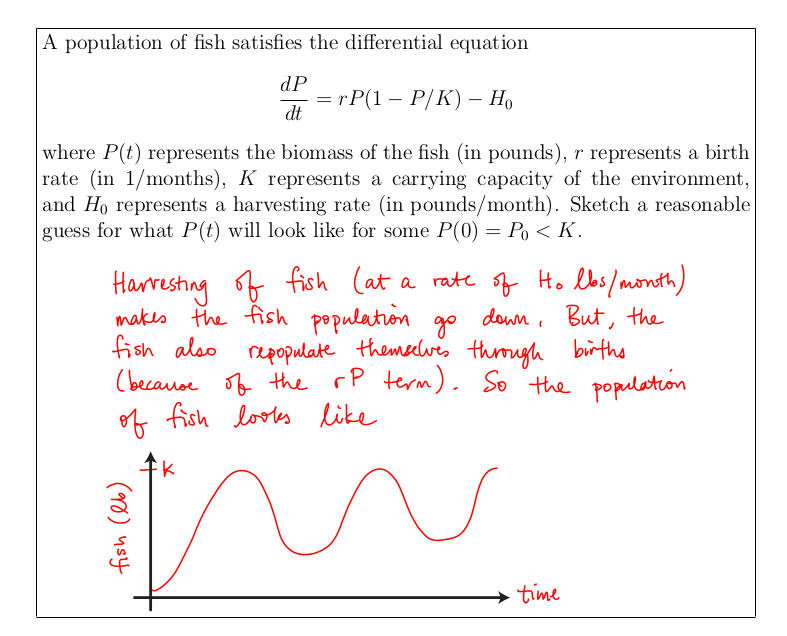
\includegraphics[scale=.5]{StudentY.png}$
\end{center}
\end{problem}
\newpage

\begin{problem}
5. \textbf{Leaky bucket}: (10 points; 5 points for (ab) and 5 points for (cd))A bucket in the shape
of a cylinder has a small hole in its bottom, through which water is leaking. Let $h(t)$
be the height of the water in the bucket, $A$ the cross-sectional area of the bucket, and a
the area of the small hole. We want to find how long it will take the bucket to empty.

\begin{center}
    
$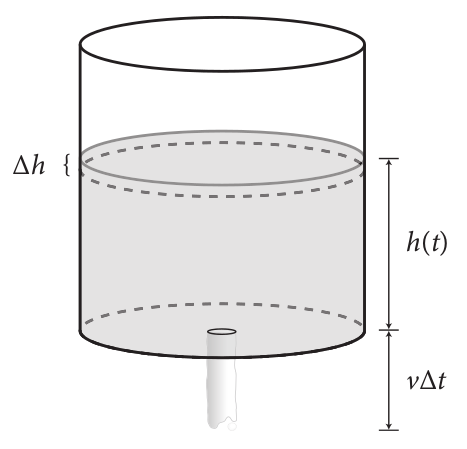
\includegraphics[scale=.4]{Bucket.png}$
\end{center}

\begin{enumerate}
    \item[(a)] Let’s assume that the water flows out of the bucket laminarly, so that the stream of
water looks roughly like a cylinder with cross-sectional area $a$ (the same as the hole).\\ 
Let $v(t)$ be the velocity of the water when it exits the bucket. It is a fact that
\begin{center}
    $av(t) = Ah'(t)$.
\end{center}
What physical principle is responsible for this fact?\\
\textbf{Hint}: In a small unit of time $\Delta t$, the height of the water in the bucket falls by $\Delta h$ and
the water at the hole travels a distance $v(t)\Delta t$, as indicated in the diagram above.
    \item[(b)] Now let’s derive a differential equation for $h(t)$ based on conservation of energy. If the
height of the water in the bucket decreases by $\Delta h$ and the density of the water is $\rho$,
the net change of potential energy in the system is$ \Delta mgh = \rho A\Delta hgh$. Since energy
cannot be created or destroyed, this decreased potential energy must be converted into
kinetic energy. The kinetic energy of the same amount of water leaving the bucket
is $\frac{1}{2}\Delta mv^2 =\frac{1}{2}\rho A\Delta hv^2$. Equating these two energies, we get$v^2 = 2gh$. Using this
information, derive a differential equation for $h(t)$.
    \item[(c)] Assume that at $t = 0$ the height of the water in the bucket is $h_0$. Define $t^\ast$ to be the time when the bucket becomes empty. Find an expression for $t^\ast$. What is $h(2t^\ast)$?(Make sure your answer is sensible.)
    \item[(d)] Suppose that at $t = 5$ you observe that the bucket is empty. Is it possible to determine
\textit{uniquely} how full the bucket was at $t = 0$? Explain why or why not.
\end{enumerate}

\end{problem}
\newpage

\begin{problem}
6. (5 points) For each IVP, what can you say about the interval forward in time from the initial
condition in which you can guarantee existence and uniqueness of the solution? Make sure
you explain why your claim is true. Use dfield1
to plot a direction field and solution curve for
each IVP. In a couple of sentences, explain how the solutions you see are or are not consistent
with the results of the theorem(s) you applied. \textbf{You do not have to analytically solve
the IVPs.}

\begin{enumerate}
    \item[(a)] $(sin t)y' + y = 2; y(5) = -2$
    \item[(b)]  $(t - 5)y' + ty = e^{-t}; y(0) = 1$
    \item[(c)] $ty' = y + ty; y(0) = 0$
\end{enumerate}
\end{problem}
\newpage

\begin{problem}
7. (5 points) In this exercise, we will prove the famous angle sum identity for sine.

\begin{enumerate}
    \item[(a)] State the angle sum identity for sine. This is the one that gives an expression for
$\text{sin}(a + b)$. You may look it up if you do not remember it.
    \item[(b)] In order to write an ODE, we have to express each side of the identity as a function of
a single independent variable. Treat b as a fixed constant, and write each side of the
equation as a function of $t$, i.e. sin$(a + b)$ becomes $y_1(t) = \text{sin}(t + b)$.
    \item[(c)] Find an IVP that is satisfied by $y_1(t)$.
    \item[(d)] Prove the angle sum identity. Hint: Consider $y_2 = \text{sin}(t) \text{cos} (b)+ \text{cos}(t)\text{sin}(b)$. Does it satisfy
your IVP from part (c)? Use existence and uniqueness.
\end{enumerate}
\end{problem}
\newpage

\begin{problem}
8. (5 points) Determine which method(s), if any, can be used to solve the following ODEs. \textbf{You
do not need to solve the ODE, but provide a brief explanation.}

\begin{enumerate}
    \item[(a)] $y' + (\text{cos}(t))y = \text{cos}(t)$
    \item[(b)] $y'+ xy^ = e^x$
    \item[(c)]$y'''+ y'\text{sin}(t) + 3y^2 = t$
    \item[(d)]$e^xy' + y = \text{tan}(x)$
\end{enumerate}
\end{problem}
\newpage

% Add pairs of problems and solutions as needed

\end{document}
